%%%%%%%%%%%%%%%%%%%%%%%%%%%%%%%%%%%%%

\section{Observational studies and sampling strategies}

%%%%%%%%%%%%%%%%%%%%%%%%%%%%%%%%%%%%

\subsection{Confounding}

%%%%%%%%%%%%%%%%%%%%%%%%%%%%%%%%%%%%

\begin{frame}
\frametitle{}

\begin{center}
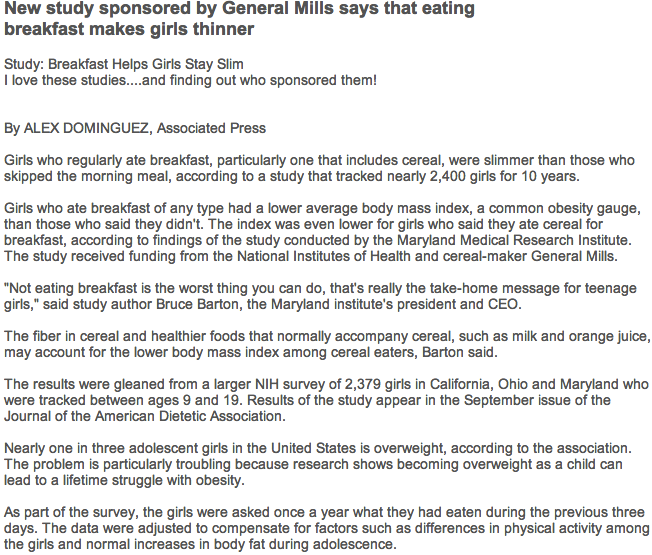
\includegraphics[width=0.80\textwidth]{1-4_obs_studies_sampling/figures/breakfast/breakfast1}
\end{center}

{\tiny \webURL{http://www.peertrainer.com/LoungeCommunityThread.aspx?ForumID=1\&ThreadID=3118}}

\end{frame}

%%%%%%%%%%%%%%%%%%%%%%%%%%%%%%%%%%%%

\begin{frame}
\frametitle{}

\dq{What type of study is this, observational study or an experiment?
{\footnotesize \textit{``Girls who regularly ate breakfast, particularly one that includes cereal, were slimmer than those who skipped the morning meal, according to a study that tracked nearly 2,400 girls for 10 years. [...] As part of the survey, the girls were asked once a year what they had eaten during the previous three days."}}
}

\soln{\onslide<2->{This is an \hl{observational study} since the researchers merely observed the behavior of the girls (subjects) as opposed to imposing treatments on them.}}

\dq{What is the conclusion of the study?}

\soln{\onslide<3->{There is an \hl{association} between girls eating breakfast and being slimmer.}}

\dq{Who sponsored the study?}

\soln{\onslide<4->{General Mills.}}

\end{frame}

%%%%%%%%%%%%%%%%%%%%%%%%%%%%%%%%%%%%

\begin{frame}[shrink]
\frametitle{3 possible explanations}

\pause

\begin{enumerate}

\item Eating breakfast causes girls to be thinner.
\begin{center}
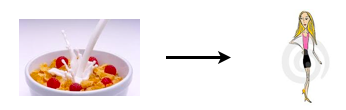
\includegraphics[width=0.5\textwidth]{1-4_obs_studies_sampling/figures/breakfast/breakfast2}
\end{center}

\pause

\item Being thin causes girls to eat breakfast.
\begin{center}
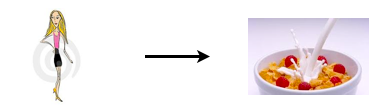
\includegraphics[width=0.5\textwidth]{1-4_obs_studies_sampling/figures/breakfast/breakfast3}
\end{center}

\pause

\item A third variable is responsible for both. What could it be? \\
An extraneous variable that affects both the explanatory and the response variable and that make it seem like there is a relationship between the two are called \hl{confounding} variables.
\begin{center}
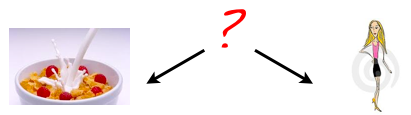
\includegraphics[width=0.5\textwidth]{1-4_obs_studies_sampling/figures/breakfast/breakfast4}
\end{center}

\end{enumerate}


{\tiny Images from: \webURL{http://www.appforhealth.com/wp-content/uploads/2011/08/ipn-cerealfrijo-300x135.jpg},  \webURL{http://www.dreamstime.com/stock-photography-too-thin-woman-anorexia-model-image2814892}.}



\end{frame}

%%%%%%%%%%%%%%%%%%%%%%%%%%%%%%%%%%%%

\begin{frame}
\frametitle{Prospective vs. retrospective studies}

\begin{itemize}

\item A \hl{prospective} study identifies individuals and collects information as events unfold. 
\begin{itemize}
\item Example: The Nurses Health Study has been recruiting registered nurses and then collecting data from them using questionnaires since 1976.
\end{itemize}

\item \hl{Retrospective studies} collect data after events have taken place.
\begin{itemize}
\item Example: Researchers reviewing past events in medical records.
\end{itemize}

\end{itemize}

\end{frame}

%%%%%%%%%%%%%%%%%%%%%%%%%%%%%%%%%%%

\subsection{Sampling strategies}

%%%%%%%%%%%%%%%%%%%%%%%%%%%%%%%%%%%

\begin{frame}
\frametitle{Obtaining good samples}

\begin{itemize}

\item Almost all statistical methods are based on the notion of implied randomness. 

\item If observational data are not collected in a random framework from a population, these statistical methods -- the estimates and errors associated with the estimates -- are not reliable.

\item Most commonly used random sampling techniques are \hl{simple}, \hl{stratified}, and \hl{cluster} sampling.

\end{itemize}

\end{frame}

%%%%%%%%%%%%%%%%%%%%%%%%%%%%%%%%%%%%

\begin{frame}
\frametitle{Simple random sample}

Randomly select cases from the population, where there is no implied connection between the points that are selected.

\begin{center}
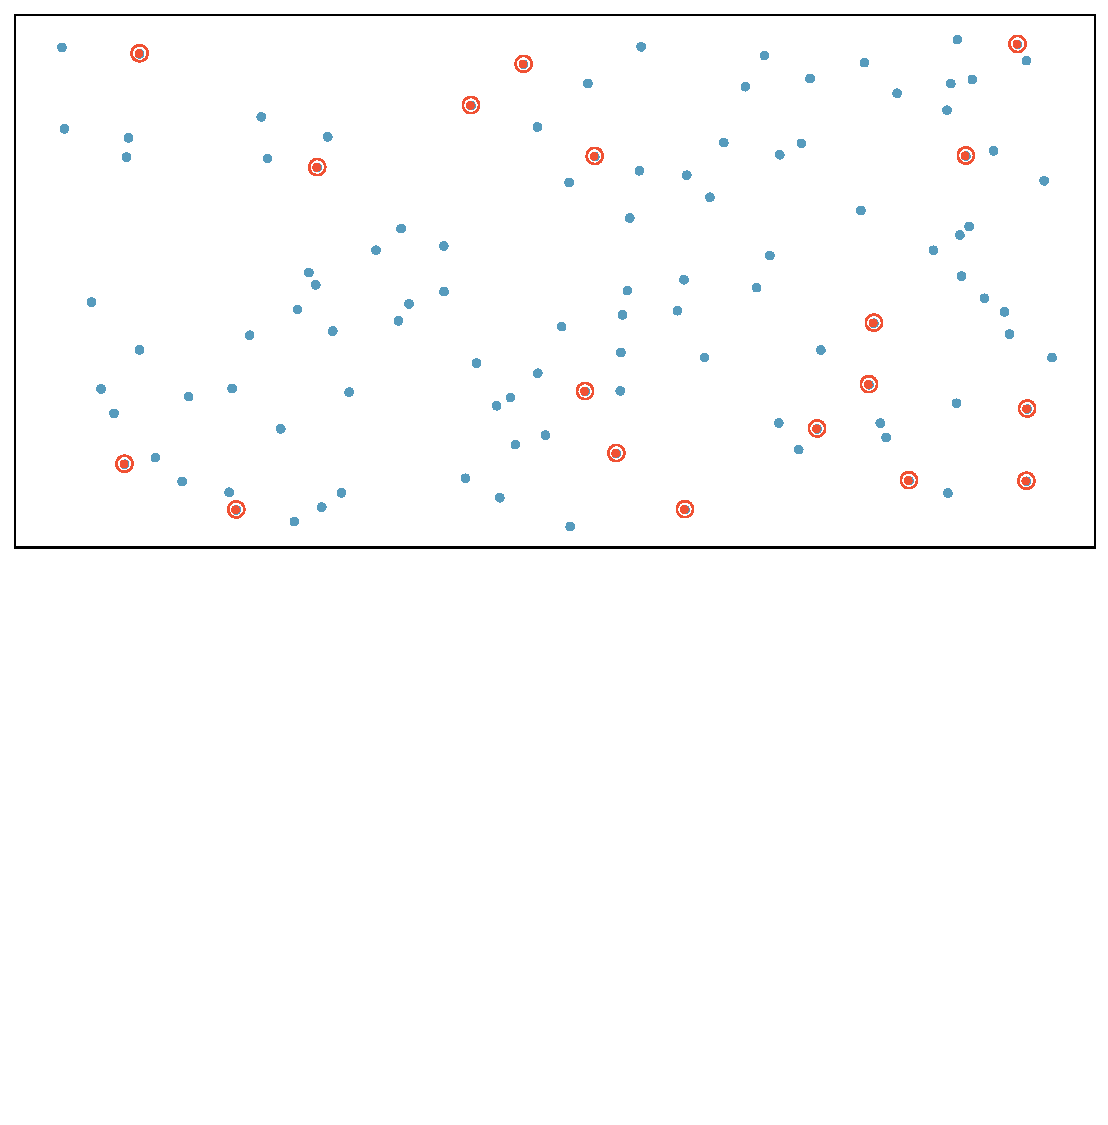
\includegraphics[width=0.9\textwidth]{1-4_obs_studies_sampling/figures/sampling_methods/simple}
\end{center}

\end{frame}

%%%%%%%%%%%%%%%%%%%%%%%%%%%%%%%%%%%%

\begin{frame}
\frametitle{Stratified sample}

\hl{Strata} are made up of similar observations. We take a simple random sample from \underline{each} stratum.

\begin{center}
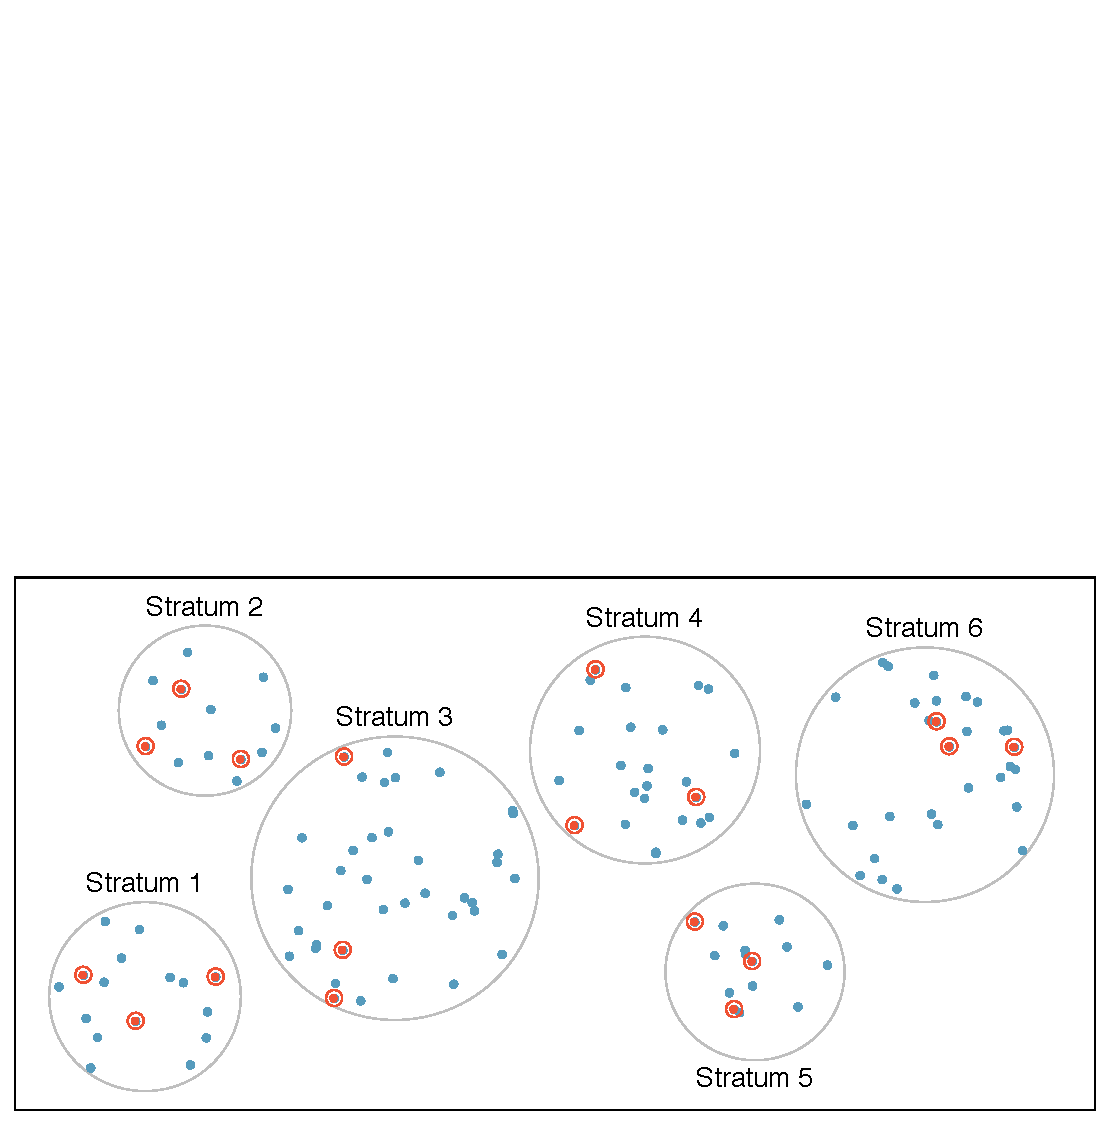
\includegraphics[width=0.9\textwidth]{1-4_obs_studies_sampling/figures/sampling_methods/stratified}
\end{center}

\end{frame}

%%%%%%%%%%%%%%%%%%%%%%%%%%%%%%%%%%%%

\begin{frame}
\frametitle{Cluster sample}

\hl{Clusters} are usually not made up of homogeneous observations. We take a simple random sample of clusters, and then sample \underline{all} observations in that cluster. Usually preferred for economical reasons.

\begin{center}
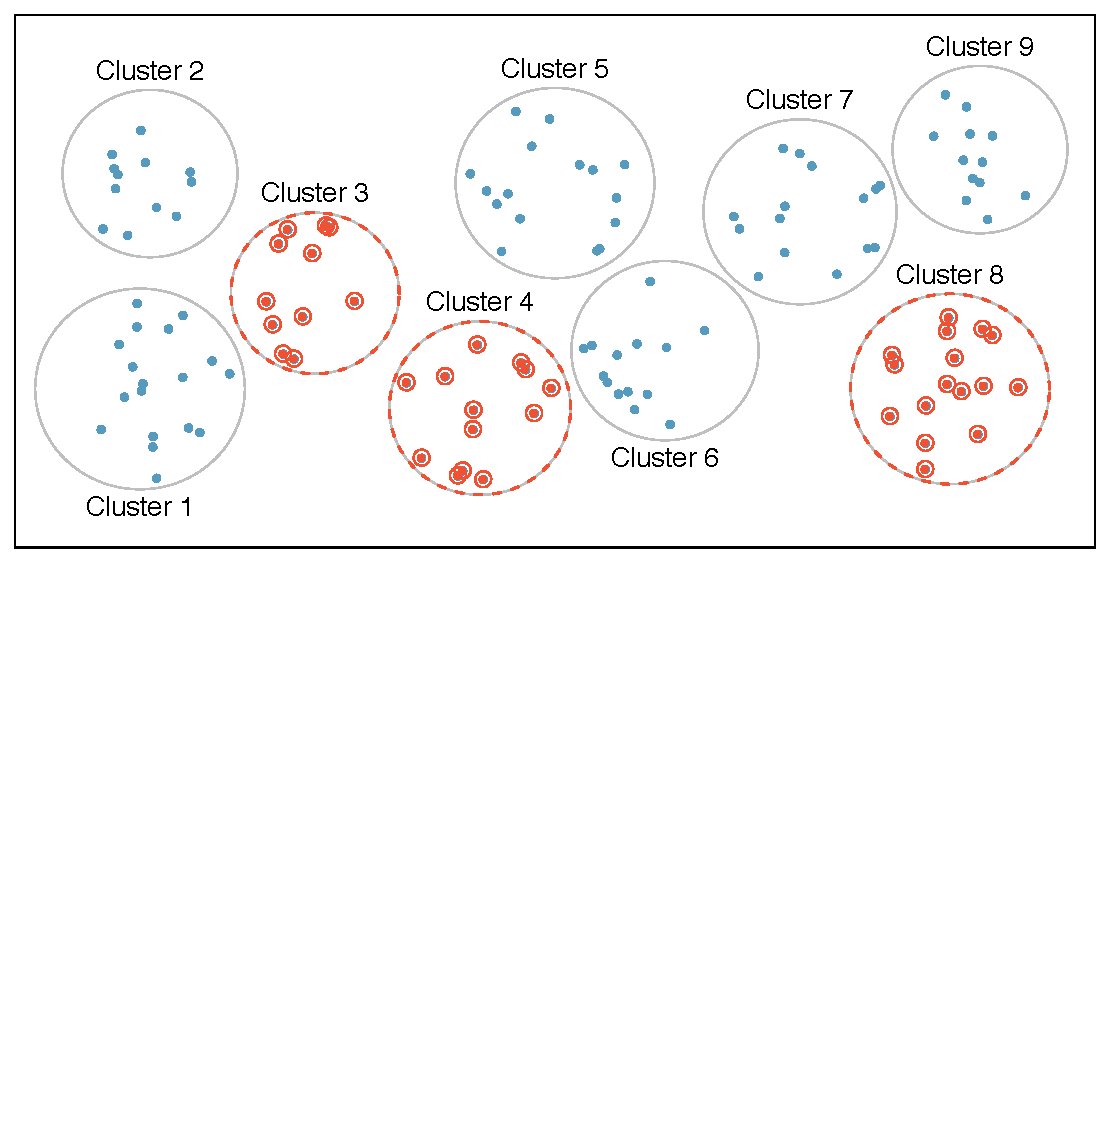
\includegraphics[width=0.9\textwidth]{1-4_obs_studies_sampling/figures/sampling_methods/cluster}
\end{center}

\end{frame}

%%%%%%%%%%%%%%%%%%%%%%%%%%%%%%%%%%%%

\begin{frame}
\frametitle{Multistage sample}

\hl{Clusters} are usually not made up of homogeneous observations.  We take a simple random sample of clusters, and then take a simple random sample of observations from the sampled clusters.

\begin{center}
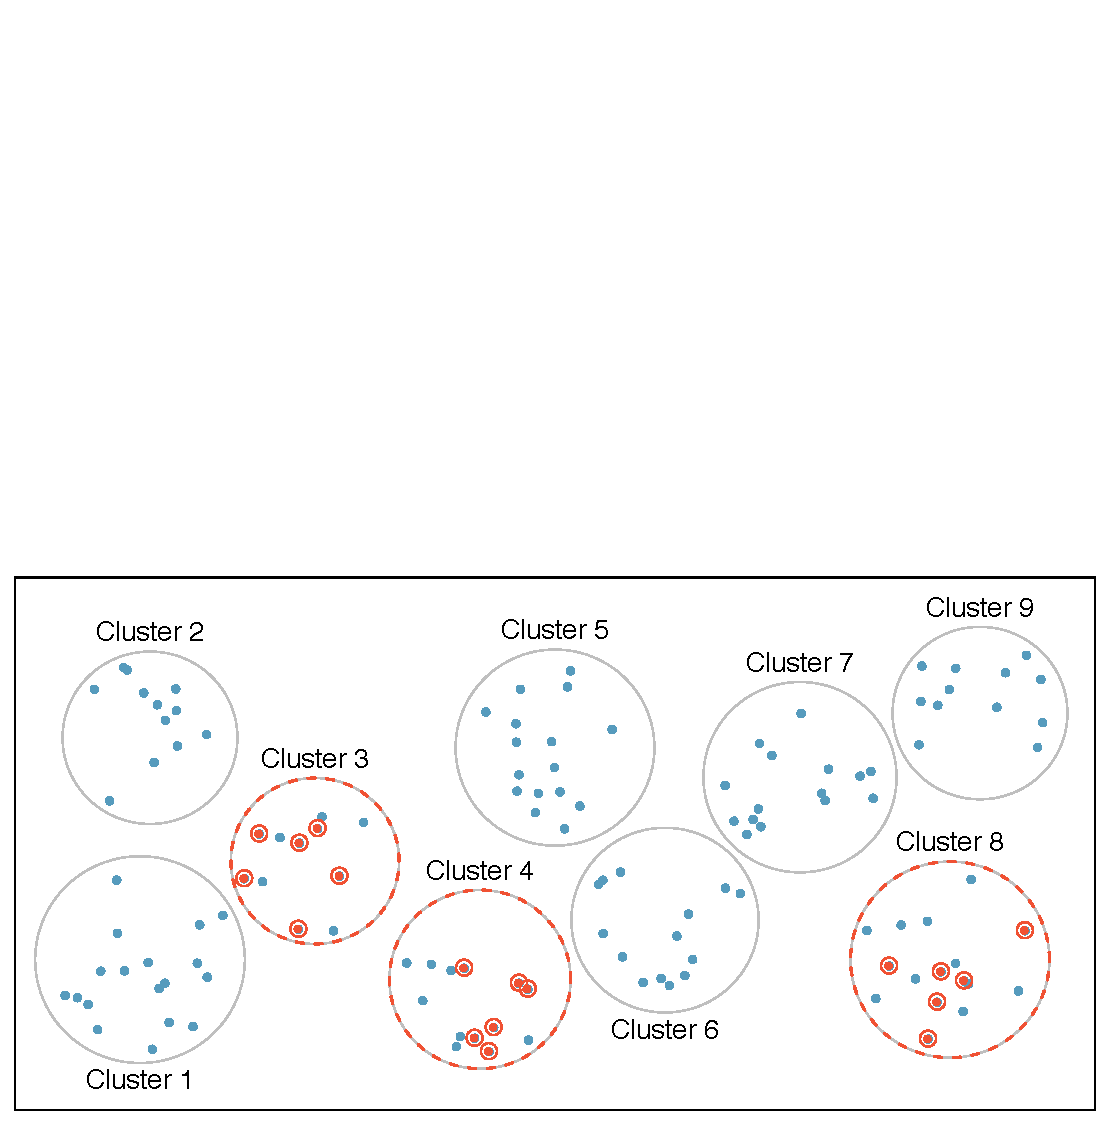
\includegraphics[width=0.9\textwidth]{1-4_obs_studies_sampling/figures/sampling_methods/multistage}
\end{center}

\end{frame}

%%%%%%%%%%%%%%%%%%%%%%%%%%%%%%%%%%%%

\begin{frame}
\frametitle{Practice}

\pq{A city council has requested a household survey be conducted in a suburban area of their city. The area is broken into many distinct and unique neighborhoods, some including large homes, some with only apartments. Which approach would likely be the \emph{least} effective?}

\begin{enumerate}[(a)]
\item Simple random sampling
\solnMult{Cluster sampling}
\item Stratified sampling
\item Blocked sampling
\end{enumerate}

\end{frame}

%%%%%%%%%%%%%%%%%%%%%%%%%%%%%%%%%%%%